\documentclass[10pt,a4paper]{article}
\usepackage[utf8]{inputenc}
\usepackage{amsmath}
\usepackage{amsfonts}
\usepackage{amssymb}

\usepackage{float}
\usepackage[table,xcdraw]{xcolor} %para usar tablas con color de fondo en las celdas
\usepackage{hyperref} %para poder poner enlaces
\usepackage{listings} %para insertar código
\usepackage{tikz}%para pintar las redes neuronales
\usepackage{color} %para poder definir y usar colores
\usepackage{soul} %para hacer los subrayados

\author{\textbf{Gustavo Rivas Gervilla}}
\title{\textcolor{deepblue}{\textbf{Titanic. Competición Kaggle.}}}
\date{}

%Configurando lstlisting para mostrar código Python con algún 	 de colores (copiado de http://tex.stackexchange.com/questions/83882/how-to-highlight-python-syntax-in-latex-listings-lstinputlistings-command) ------------------------------
% Custom colors
\definecolor{deepblue}{rgb}{0,0,0.5}
\definecolor{deepred}{rgb}{0.6,0,0}
\definecolor{deepgreen}{rgb}{0,0.5,0}
\definecolor{light-gray}{gray}{0.85}
\definecolor{comment-gray}{gray}{0.65}
\definecolor{light-green}{rgb}{0.66,1,0.5}
\definecolor{light-yellow}{rgb}{1,1,0.4}

% Default fixed font does not support bold face
\DeclareFixedFont{\ttb}{T1}{txtt}{bx}{n}{8} % for bold
\DeclareFixedFont{\ttm}{T1}{txtt}{m}{n}{8}  % for normal

%Configuración de los listings
\lstset{
	language=Python,
	basicstyle=\ttm,
	otherkeywords={self},             % Add keywords here
	keywordstyle=\ttb\color{deepblue},
	emph={MyClass,__init__},          % Custom highlighting
	emphstyle=\ttb\color{deepred},    % Custom highlighting style
	stringstyle=\color{deepgreen},
	frame=tb,                         % Any extra options here
	showstringspaces=false,            % 
	commentstyle=\ttm\color{comment-gray}, % Custom comment style
}
%--------------------------------------------------------------------------------

\newcommand{\emp}[1]{\sethlcolor{light-yellow}\hl{\texttt{#1}}} %Comando para poner código inline
\newcommand{\code}[1]{\sethlcolor{light-gray}\hl{\texttt{#1}}} %Comando para poner código inline
\newcommand{\archive}[1]{\sethlcolor{light-green}\hl{\texttt{#1}}} %Comando para resaltar nombres de archivos
\renewcommand\tablename{Tabla} %Cambiar el nombre de las tablas
\renewcommand\figurename{Figura} %Cambiar el nombre de las tablas
\renewcommand{\contentsname}{Índice} %Cambiar el nombre de la ToC

\usepackage{pdfpages}

\begin{document}
\maketitle

\begin{center}
  \textbf{Nombre del equipo: }Gustavo Rivas Gervilla\\
  \textbf{Ranking global: }TODO\\
  \textbf{Puntuación: }TODO
\end{center}

\newpage

\tableofcontents

\newpage

\section{Introducción}

En este trabajo se va a trabajar con el dataset del Titanic, un conjunto de datos en el que se plantea un \textbf{problema de clasificación}, dadas una serie de características de un pasajero, que enumeraremos en la siguiente sección, se tendrá que decidir si el pasajero sobrevivió o no a la catastrofe. En primer lugar, como toma de contacto con el dataset y también para tomar algunas ideas que aplicar al conjunto de datos, se han realizado dos tutoriales con planteamientos similares, ambos realizan un preprocesamiento parecido a los datos y emplean Random Forest como algoritmo final de clasificación, después de probar otros modelos como puede ser uno basado en un árbol de decisión o simplemente suponer que todas las mujeres sobrevivieron y que todos los hombres perecieron. La realización de estos dos tutoriales se adjunta en esta memoria a modo de apéndices.\\

\section{Exploración de datos}

En primer lugar vamos a presentar el conjunto de datos que tenemos, disponemos de 891 instancias en el conjunto de entrenamiento y 418 en el conjunto de test. Estas instancias presentan el siguiente conjunto de atributos:

\begin{enumerate}
\item \textbf{PassengerId: } identificador del pasajero.
\item \textbf{Pclass: } la clase en la que embarcó.
\item \textbf{Name:} el nombre del pasajero.
\item \textbf{Sex: } sexo del pasajero.
\item \textbf{Age: } edad del pasajero.
\item \textbf{SibSp: } número de hermanos/esposos/esposas del pasajero que viajaban también a bordo.
\item \textbf{Parch: } número de padres/hijos del pasajero que viajaban también a bordo.
\item \textbf{Ticket: } número o identificador del ticket de embarque del pasajero.
\item \textbf{Fare: } lo que pagó el pasajero por su pasaje.
\item \textbf{Cabin: } camarote(s) en el(los) que viajó el pasajero.
\item \textbf{Embarked: } puerto desde el que embarcó. C = Cherbourg, Q = Queenstown, S = Southampton.
\item \textbf{Survived: } el pasajero murió (0) o sobrevivió (1). La variable a predecir y que por tanto no está presente en las intancias del conjunto de test.
\end{enumerate}

Lo primero que hemos hecho ha sido estudiar si contábamos con valores perdidos. Gracias a los tutoriales notamos que hay algunos atributos que, si bien no presentan valores perdido (\textbf{NA}), contienen una cadena vacía lo que se podría considerar también un valor perdido, y por lo tanto esto también se tendrá en cuenta en la fase de preprocesamiento. Tras este análisis vemos que la mayoría de valores perdidos están en el atributo \textbf{Age}, también hay algún valor perdido en el \textbf{Embarked} y en \textbf{Cabin}.\\

Vamos a ver ahora la primera gráfica sobre nuestro conjunto de datos, lo que vamos a reflejar en esta gráfica es el desequilibrio entre las dos clases (549 muertos y 342 sobrevivientes), aunque no se trata de un desequilibrio demasiado grande lo trataremos en la fase de preprocesamiento y trataremos de comparar distintas técnicas de balanceo de clases según su rendimiento para un algoritmo determinado:

\begin{figure}[H]
  \centering
  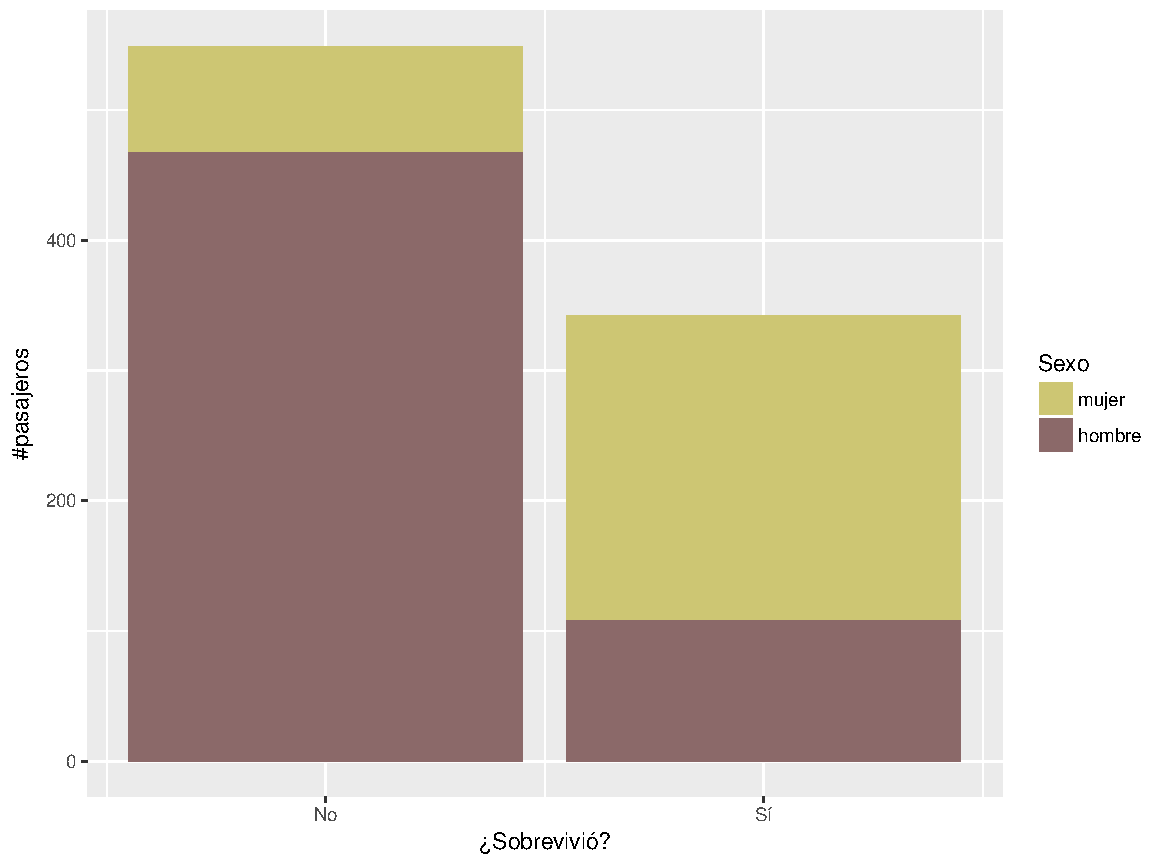
\includegraphics[width=\textwidth]{imgs/imbalanced}
  \caption{Desbalanceo entre clases}
\end{figure}

En la gráfica anterior también mostramos en qué proporción sobreviven hombres y mujeres en el conjunto de entrenamiento. Como podemos ver son las mujeres las que en su mayoría sobrevivieron mientras que los hombres tuvieron menos posibilidades, recordemos que durante el accidente del Titanic se estableció la política de evacuar a mujeres y niños en primer lugar con lo que esta gráfica parece acorde a ello. Este hecho nos lleva, en el tutorial de Trevor Stephens, a plantear el modelo sexista.
\appendix

\section{Tutorial ``Exploring Survival on the Titanic'' de Megan Risdal}

%\includepdf[pages=-]{StephensTitanicTutorial}

A modo de introducción tanto al dataset como a la plataforma Kaggle vamos a realizar este tutorial que nos servirá para dar una primera solución al problema que se nos plantea con este dataset. También, y simplemente por conocer esta herramienta, se ha optado por realizar este tutorial desarrollando un aplicación web Shiny. El fichero tiene extensión de Rmarkdown, algo que ya he usado, con lo cual no debería ser muy complicado usar esta utilidad que ofrece Rstudio.

\subsection{Preprocesamiento}

Lo primero que observamos es el uso de la función \code{bind\_rows} del paquete \code{dplyr}, lo que hacemos con esta función es unir los datasets de train y test en uno solo, la diferencia entre esta función y usar por ejemplo \code{rbind} es que nos facilita el trabajo, ya que mientras que \code{rbind} nos da un error al no tener ambos datasets el mismo número de columnas (el conjunto de test no contiene la clase a la que pertenece cada una de las instancias ya que es lo que hemos de predecir de cara a la competición), con \code{bind\_rows} lo que hace es unir ambos e insertar \textbf{NA} en aquellos atributos que no están presentes en el dataset de test, la clase de los pasajeros.\\

En el tutorial realiza una pequeña exploración sobre el conjunto total de instancias del problema haciendo uso de la función \code{str} aunque esto no nos aporta información acerca de la semántica de cada uno de los atributos del dataset, estos son los siguientes:

\begin{enumerate}
\item Survived: la clase a predecir. Sobrevivió (1) o murió (0).
\item Pclass: la clase del pasaje.
\item Name: el nombre del pasajero.
\item Sex: sexo del pasajero.
\item Age: edad del pasajero.
\item SibSp
\item Parch
\item Ticket
\item Fare: 
\item Cabin: número de camarote.
\item Embarked: puerto en el que embarcó.
\end{enumerate}

\subsection{Subiendo resultados a Kaggle}

A modo de ejercicio lo que he hecho ha sido generar simplemente una predicción completamente aleatoria, de este modo podremos testear rápidamente el sistema de subida a la plataforma Kaggle y además tener un punto de referencia más para comparar los distintos experimentos que realicemos. Con esta predicción hemos obtenido un score de \textbf{0.43541}. Observemos que hemos puesto el atributo \code{quote} de la función \code{write.csv} de modo que el nombre de las columnas del dataset se introduzcan sin ir entre comillas dobles, de otro modo Kaggle no aceptaría el submisión.

Tras el tutorial de Riscal pos \textbf{989} accuracy \textbf{0.80383}

Tras aplicar Xgboost al dataset de Riscal \textbf{0.77990}.

\end{document}